\section*{4 Data}

\indent My primary data source is DIME Public version 4.0 (Bonica), which ``contains over 850 million itemized political contributions made by individuals and organizations to local, state, and federal elections covering from 1979 to 2024'' \cite{bonica2024}. Given the magnitude of the data, I restricted my attention to U.S.\ House elections in cycles 2000 -- 2022 (2024 data was incomplete, as discovered during my cleaning process). Initial filtering uses DuckDB to select:

\begin{enumerate}
	\item Table \textbf{candDB}: federal House (\texttt{seat = `federal:house'}), \texttt{cycle} between 2000 and 2024, non-null \texttt{bonica\_rid}
	\item Table \textbf{contribDB}: matching \texttt{bonica\_rid}, \texttt{seat = `federal:house'}, \texttt{date} between 1998-01-01 and 2024-12-31\footnote{The date Jan 1, 1998 was used in attempt to capture pre-2000 contribution data for the 2000 election cycle.}\
	\item Table \textbf{donorDB}: matching \texttt{bonica\_cid} in contributions table
\end{enumerate}

\indent Variable pruning retains nineteen candidate-table fields: \texttt{bonica\_rid, bonica\_cid, \\ cycle, party, district, ico\_status, num\_givers, total\_unitemized, \\ total\_disbursements, total\_receipts, total\_indiv\_contribs, gwinner, \\ total\_pac\_contribs, total\_contribs\_from\_candidate, district\_pres\_vs, \\ total\_party\_contribs, ind\_exp\_support, ind\_exp\_oppose} \text{ and } \texttt{gen\_vote\_pct}. Nine contribution-table fields are kept: \texttt{cycle} (to validate the election year in the candidate table), \texttt{transaction\_type, date, amount, bonica\_rid, bonica\_cid, \\ contributor\_type, is\_corp,} \text{ and } \texttt{election\_type}. All other columns within these tables are dropped, and the donor table is removed entirely.\footnote{No variables related to my objective were contained within this table.} A description of all variables, as well as how they were transformed for modeling, if applicable, is located in Appendix B.

\indent Joining candidate and contribution tables yields approximately 97.4 million rows. I kept only general-election observations (\texttt{election\_type = `G'}), drop rows with null \texttt{gen\_vote\_pct} or \texttt{gwinner}, and then drop remaining nulls in \texttt{transaction\_type, date, contributor\_type}, and \texttt{district\_pres\_vs}, leaving 9,430,440 observations. I then converted \texttt{is\_corp: `corp' $\xrightarrow{}$} 1, NULL $\xrightarrow{}$ 0.

\indent Finally, I attached a CPI deflator table (base 2024 USD), adjusted all monetary columns accordingly, computed each contribution's \texttt{days\_before} (days between contribution date and election date), dropped original money and date fields, and encoded categorical variables: \texttt{contributor\_type} $\xrightarrow{}$ binary, one-hot for \texttt{ico\_status}, and frequency encoding for \texttt{transaction\_type}. The resulting {\tt house} table is ready for aggregation and modeling.

\subsection*{Visual Analysis}

Figure~\ref{fig:dist} depicts the distribution of logarithmic-scaled contributions in the cleaned table. It illustrates the heavy right tail --- most contributions are small, but a few very large gifts stretch the distribution. This indicates that contributions made by individuals may play a greater role in affecting election outcomes compared to committees, loans, and candidate self-financing.

\begin{figure}[h]
	\centering
	\includegraphics[width = 0.7\linewidth]{../Figures/amount_dist.pdf}
	\caption{Log-scale Contribution Relative Frequency Distribution}
	\label{fig:dist}
\end{figure}

Figure~\ref{fig:trend} depicts total U.S.\ House campaign contributions (in 2024 USD billions) by cycle. An upward trend is apparent, demonstrating the rise in campaign financing over recent years and thus the value in quantifying how a candidate's likelihood of victory changes as donations increase.

\begin{figure}[!t]
	\centering
	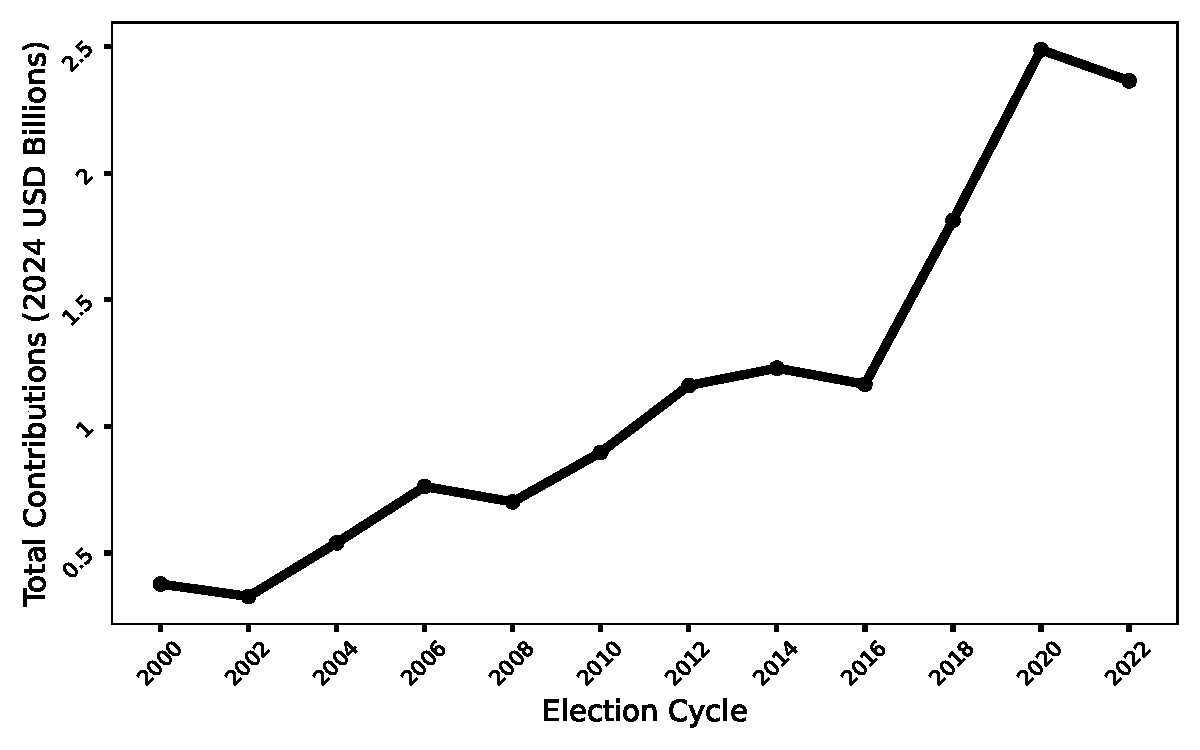
\includegraphics[width = 0.7\linewidth]{../Figures/cycle_spending_trend.pdf}
	\caption{Total U.S.\ House Campaign Contributions by Cycle (2024 USD Billions)}
	\label{fig:trend}
\end{figure}
